% Copyright 2014 James P. Fairbanks
% project presentation for the MATH6443
% Discussing the work on updating QR factorization under sparse updates

\documentclass{beamer}

% There are many different themes available for Beamer. A comprehensive
% list with examples is given here:
% http://deic.uab.es/~iblanes/beamer_gallery/index_by_theme.html
% You can uncomment the themes below if you would like to use a different
% one:
%\usetheme{AnnArbor}
%\usetheme{Antibes}
%\usetheme{Bergen}
%\usetheme{Berkeley}
%\usetheme{Berlin}
%\usetheme{Boadilla}
%\usetheme{boxes}
%\usetheme{CambridgeUS}
%\usetheme{Copenhagen}
%\usetheme{Darmstadt}
%\usetheme{default}
%\usetheme{Frankfurt}
%\usetheme{Goettingen}
%\usetheme{Hannover}
%\usetheme{Ilmenau}
%\usetheme{JuanLesPins}
%\usetheme{Luebeck}
%\usetheme{Madrid}
%\usetheme{Malmoe}
%\usetheme{Marburg}
%\usetheme{Montpellier}
%\usetheme{PaloAlto}
\usetheme{Pittsburgh}
%\usetheme{Rochester}
%\usetheme{Singapore}
%\usetheme{Szeged}
%\usetheme{Warsaw}
\usecolortheme{lily}
\title{Updating QR Factorization Under Sparse Updates.}

% A subtitle is optional and this may be deleted
%\subtitle{}
\author{James Fairbanks\inst{1} \and Domenic Carr\inst{2}}
% - Give the names in the same order as the appear in the paper.
% - Use the \inst{?} command only if the authors have different
%   affiliation.

\institute[Georgia Tech] % (optional, but mostly needed)
{
  \inst{1}%
  School of CSE
  \and
  \inst{2}%
  School of ECE
  }
% - Use the \inst command only if there are several affiliations.
% - Keep it simple, no one is interested in your street address.

% - Either use conference name or its abbreviation.
% - Not really informative to the audience, more for people (including
%   yourself) who are reading the slides online

% If you have a file called "university-logo-filename.xxx", where xxx
% is a graphic format that can be processed by latex or pdflatex,
% resp., then you can add a logo as follows:

% \pgfdeclareimage[height=0.5cm]{university-logo}{university-logo-filename}
% \logo{\pgfuseimage{university-logo}}

% Let's get started
\begin{document}

\begin{frame}
  \titlepage
\end{frame}


\begin{frame}{Overview}{}
  \begin{itemize}
  \item 
    In a least squares problem, the data might change. If the change occurs in a sparse way the QR decomposition can be updated faster than recomputation.
    \item
    First goal: Present a method that leverages the specialized structure of the update to accelerate QR computation
    \item Second goal: Experimentally determine the crossover point for different $m$, $n$, $k$ values at which recomputation is faster than  specialized updating.
  \end{itemize}
\end{frame}

% You can reveal the parts of a slide one at a time
% with the \pause command:
\begin{frame}{Updating Algorithms} The total number of fill-in entries eliminated is 
\[ Lazy = \sum_{j=1}^k \sum_{t=1}^j (i_{j+1} - i_{j} - t) = \sum_{j=1}^k j(i_{j+1}-i_{j} - \frac{j+1}{2})
\]
This is called the lazy elimination strategy because we defer elimination of fill-in entries until the last possible moment.

The eager strategy eliminates fill-in as soon as it is created. 
The total number of fill-in entries removed is
\[ Eager = \sum_{j=1}^k j(n - i_{j}) = n\sum_{j=1}^k j - \sum_{j=1}^k ji_j = \frac{nk(k+1)}{2} - \sum_{j=1}^k i_j
%\sum_{j=1}^k n-i_j + \sum_{j=1}^k j(i_{j+1}-i_{j} - \frac{j+1}{2}
\]
Both methods must eliminate the original nonzeros which are counted by $\sum_{j=1}^k n-i_j $. 

\end{frame}

\begin{frame}{Crossover Theory} 
For a fixed $m$ large enough, the Householder based methods are cubic in $n$ and the sparse updating methods are quadratic in $n$ because we need to accumulate $Q$. 
Thus making this simplification we can model the performance ratio as
\begin{equation}\label{eqn:model}
    r_e(m,n,k) = \frac{C_m n^3}{n^2k} = \frac{Cn}{k}
\end{equation}
The relationship between $m$ and $n$ is accounted for in the dependence of $C_m$ on $m$.
When $r_e=1$ the two methods will take the same amount of time, and the $k$ for which this occurs is called the break even point.
\end{frame}

\begin{frame}{Results}
\newcommand{\plotwidth}{2.2in} %width of the plots in the tabular below
%insert the plots of crossover points and speedup ratios
\begin{figure}
\begin{tabular}{cc}
%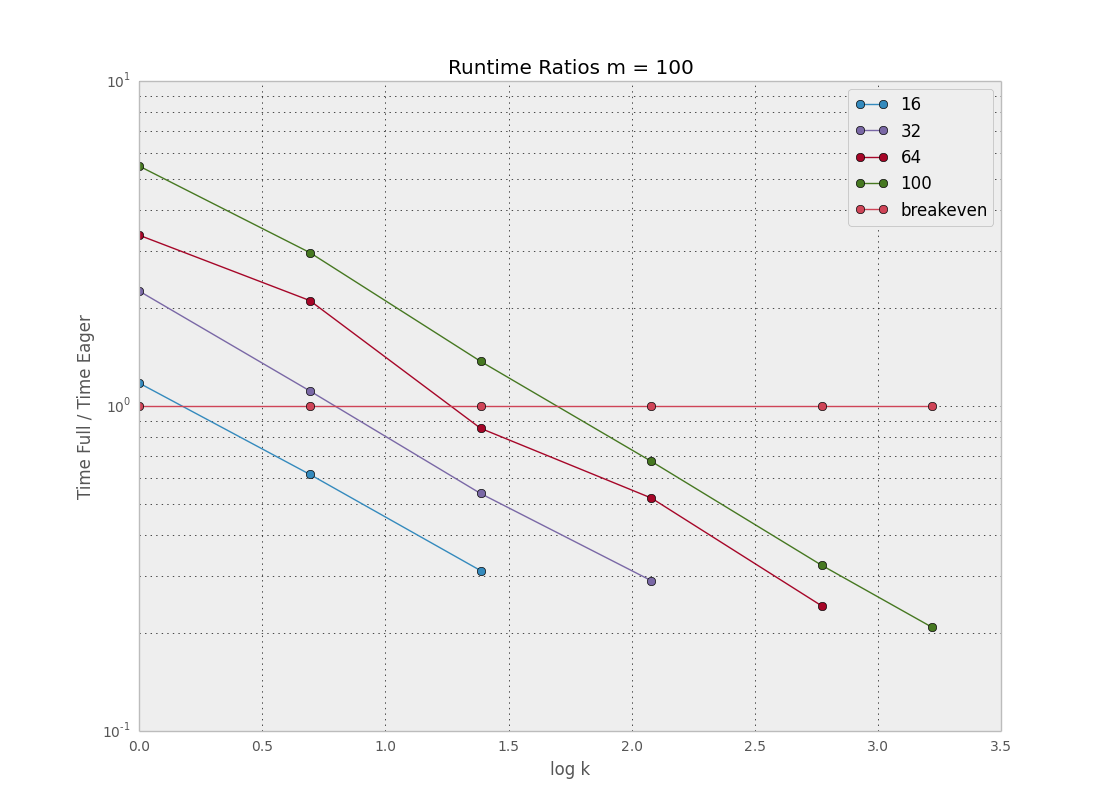
\includegraphics[width=\plotwidth]{tratio100.png} & 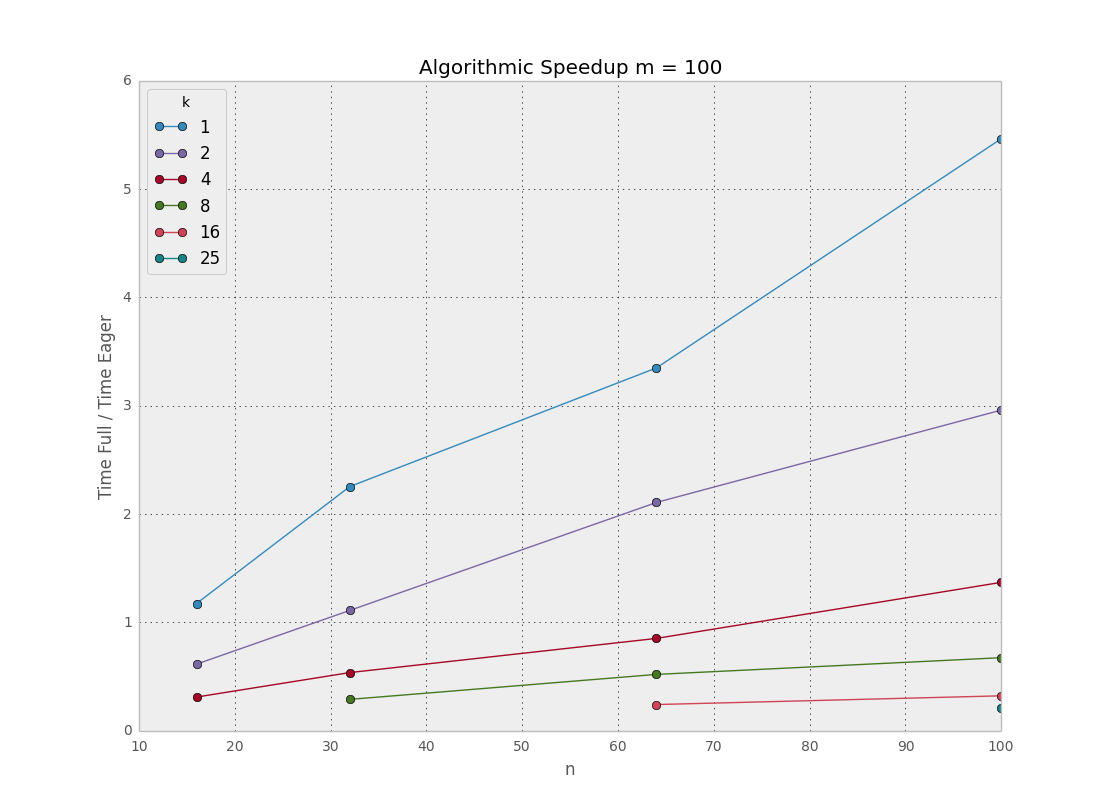
\includegraphics[width=\plotwidth]{tratioarc100.png} \\
%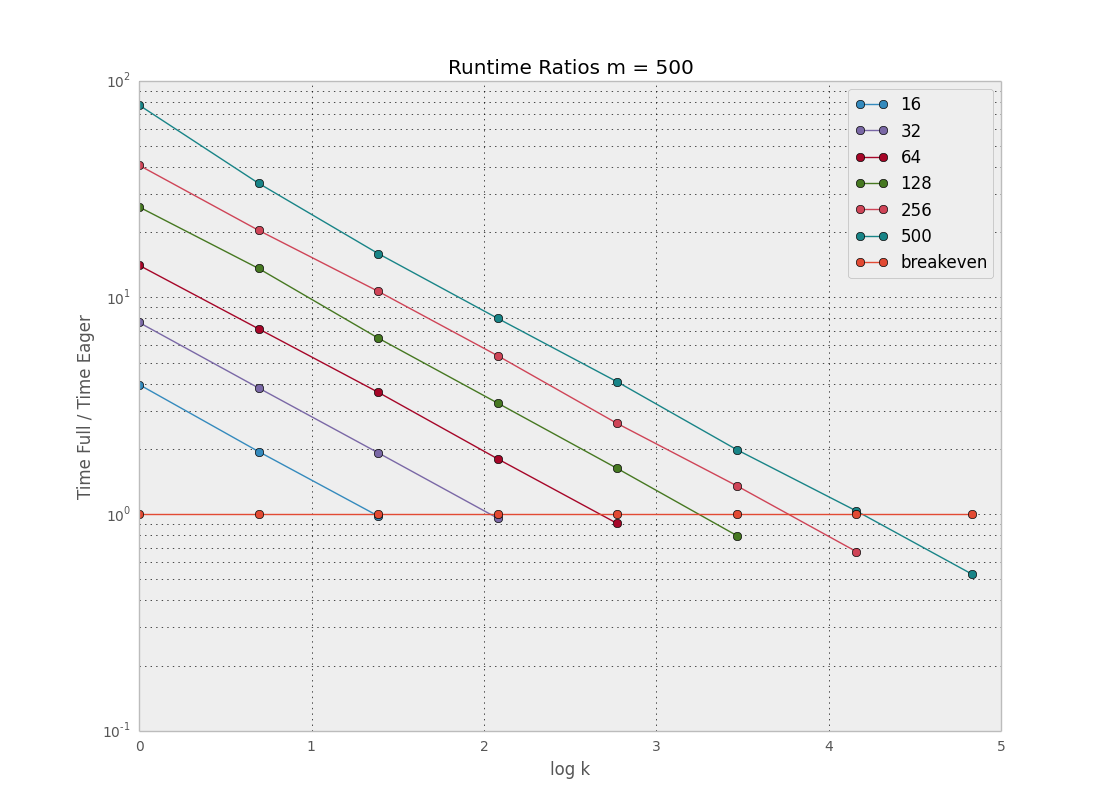
\includegraphics[width=\plotwidth]{tratio500.png} & 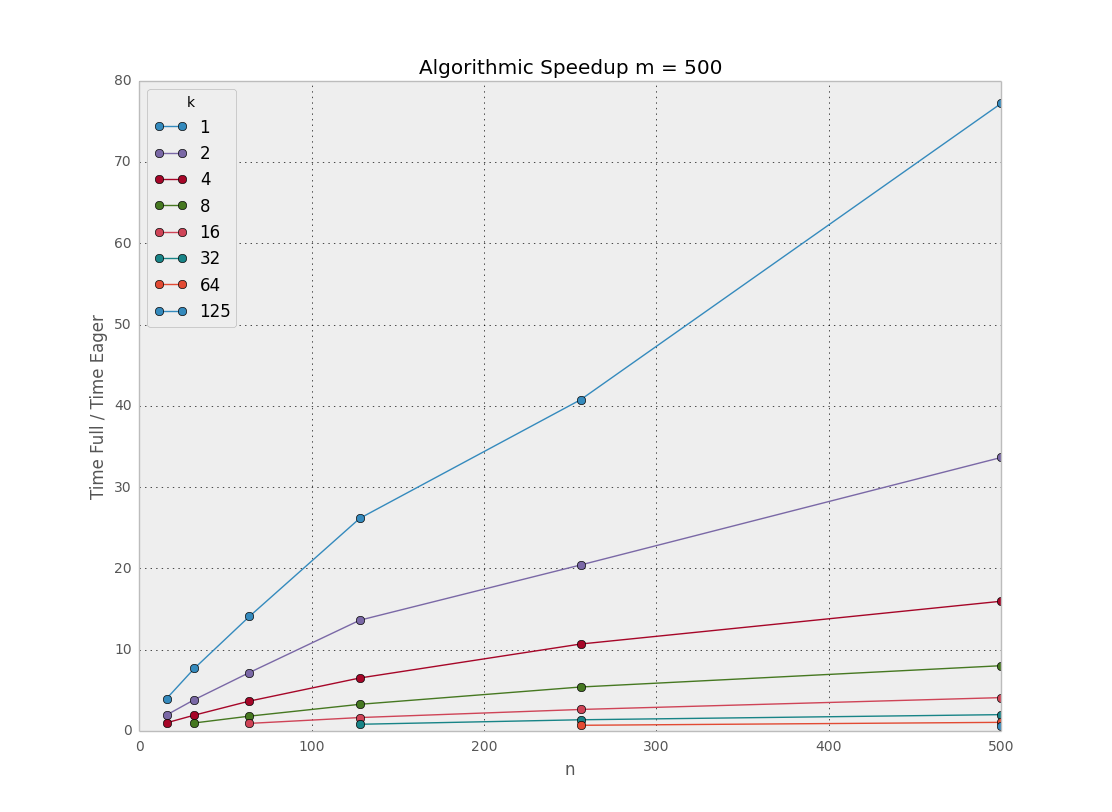
\includegraphics[width=\plotwidth]{tratioarc500.png} \\
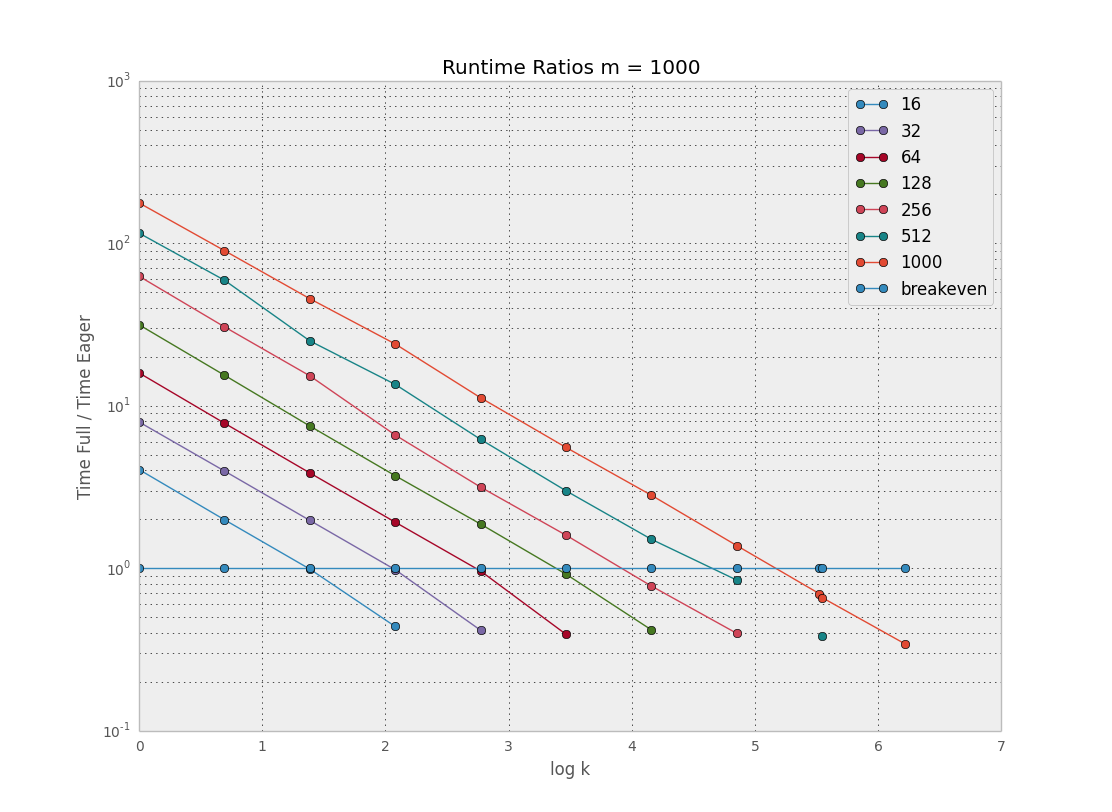
\includegraphics[width=\plotwidth]{tratio1000.png} & 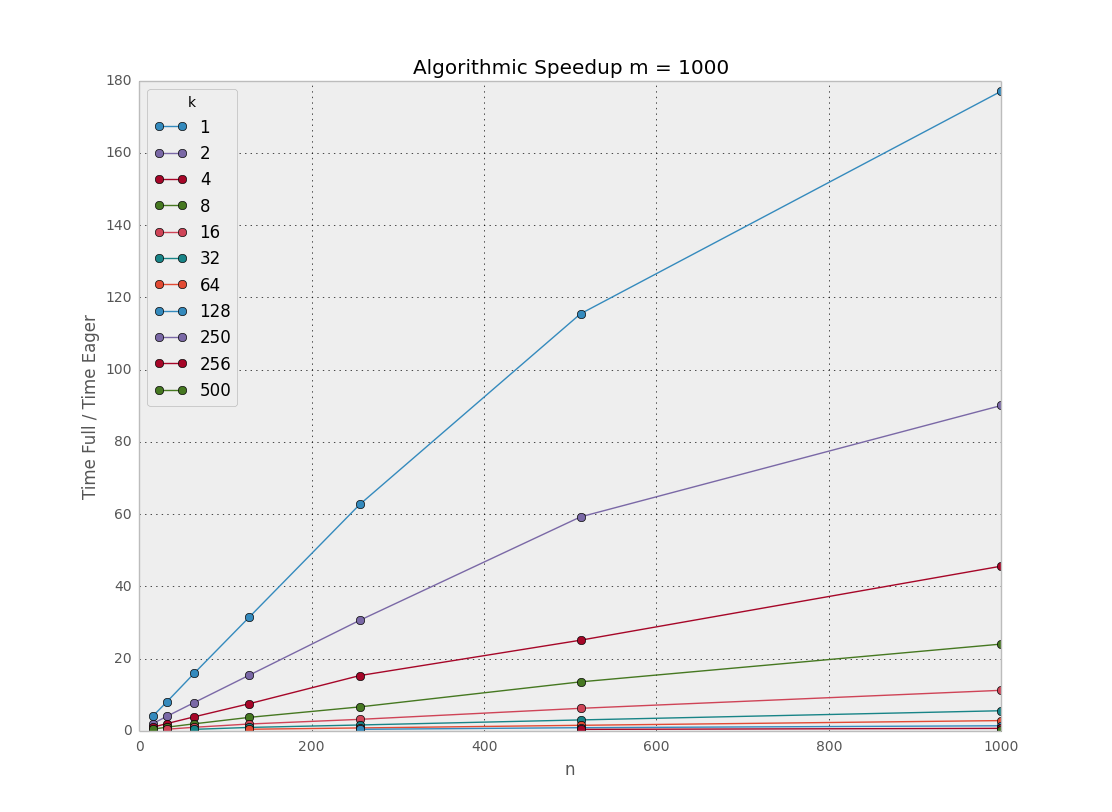
\includegraphics[width=\plotwidth]{tratioarc1000.png}\\
\end{tabular}
\caption{$r_e$ as a function of $k$ (left) and as a function of $n$ (right) }
% \label{fig:100plot}
% \label{fig:500plot}
\label{fig:1000plot}
\end{figure}

\end{frame}

\end{document}


